\section{Numerical Results}
\label{intro:numerical}

Following our analysis in $\S 5.3$, we considered a wavenumber $p=r$ and defined the Dirichlet and Neumann traces
\begin{subequations}
\label{Eqn:MMS:Input}
\begin{gather}
\xi_r^u(x) := u_r(x,g(x)),
\quad
\nu_r^u(x) := -\partial_N u_r(x,g(x)),
\\
\xi_r^w(x) := w_r(x,g(x)),
\quad
\nu_r^w(x) := \partial_N w_r(x,g(x)).
\end{gather}
From these we defined the two--layer data to be provided to our algorithm
\be
\zeta_r := \xi_r^u - \xi_r^w,
\quad
\psi_r := -\nu_r^u - \tau^2 \xi_r^w,
\ee
\end{subequations}
cf. $(5.4)$. We selected the profile
\be
\label{Eqn:Params:Geom}
g(x) = \Eps f(x) = \Eps \left( \frac{\cos(4x)}{4} \right),
\ee
with the following physical parameters
\be
d = 2 \pi,
\quad
\alpha = 0,
\quad
\epsilon^u = 1,
\quad
\epsilon^w = 1.1,
\quad
r = 4,
\quad
A_r = 5,
\quad
B_r = 3,
\label{Eqn:Params:Phys}
\ee
in TM polarization, and the numerical parameters
\be
\label{Eqn:Params:Num}
N_x = 32,
\quad
N_z = 32,
\quad
a = 1,
\quad
b = -1.
\ee
With a rescaling of the frequency (e.g., via a change of the time
variable, $t' = t/c_0$) we arrange for $c_0=1$ and considered the base frequency
\bes
\uomega_1 = 3/2,
\ees
and filling fraction $\sigma=0.99$. To illuminate the behavior of our scheme we studied four choices of
the numerical parameter
\bes
N = M = 4, 8, 12, 16,
\ees
and the physical quantities
\bes
\Eps = 10^{-2}, 10^{-4}, 10^{-6}, 10^{-8},
\ees
in $(5.26)$.
For this we supplied the ``exact'' input data, $\{ \zeta_r, \psi_r \}$,
from $(5.25)$
to our HOPS/AWE algorithm to simulate solutions of the two--layer problem
giving $\{ \xi_r^{u,\text{approx}}, \xi_r^{w,\text{approx}}\}$.
We compared this with the ``exact'' solutions
$\{ \xi_r^{u,\text{exact}}, \xi_r^{w,\text{exact}} \}$
and computed the relative error
\bes
\text{Error}_{\text{rel}} :=
  \frac{\SupNorm{\xi_r^{u,\text{exact}} - \xi_r^{u,\text{approx}}}}
  {\SupNorm{\xi_r^{u,\text{exact}}}}.
\ees
The results of our simulations are shown in 
Figures $13$ and $14$. More specifically,
Figure~$13$ displays both the rapid and stable decay of the 
relative error for fixed $N$ and $M$, and how this rate of decay
improves as $(\Eps,\delta)$ decrease. Figure~$14$ shows
both how the error shrinks as $(\Eps,\delta)$ become smaller, and that
this rate is enhanced as both $N$ and $M$ are increased.
%
% Begin Figure: Strain Plots: Error versus N and Eps (IIO)
%
%\begin{figure}[hbt]
\vspace{-19mm}
\begin{figure}[H]
\centering
    \subfloat[\centering $N=M=4, \varepsilon=10^{-2}$ ]
    {{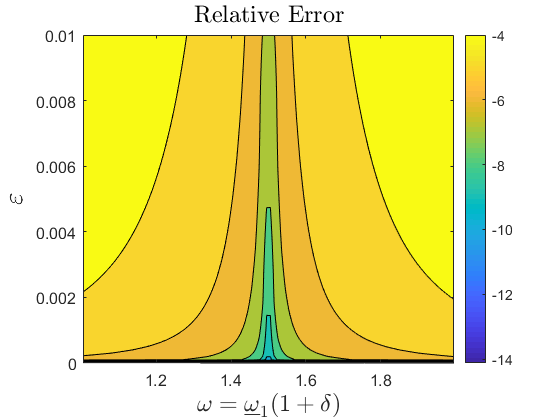
\includegraphics[width=7.6cm]{sections/5_method_of_maufactured_solutions/MMS_N_M_4_Upper_Field_Eps_1e-2.png} }}
    \subfloat[\centering $N=M=4, \varepsilon=10^{-4}$ ]
    {{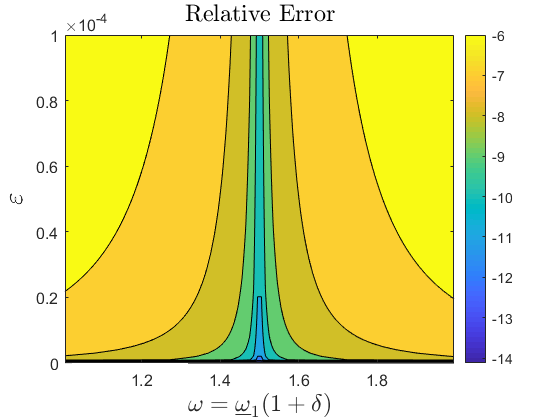
\includegraphics[width=7.6cm]{sections/5_method_of_maufactured_solutions/MMS_N_M_4_Upper_Field_Eps_1e-4.png} }}
    \\
    \subfloat[\centering $N=M=4, \varepsilon=10^{-6}$ ]
    {{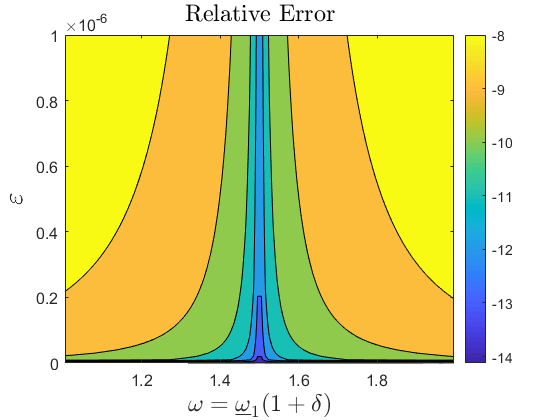
\includegraphics[width=7.6cm]{sections/5_method_of_maufactured_solutions/MMS_N_M_4_Upper_Field_Eps_1e-6.png} }}
    \subfloat[\centering $N=M=4, \varepsilon=10^{-8}$ ]
    {{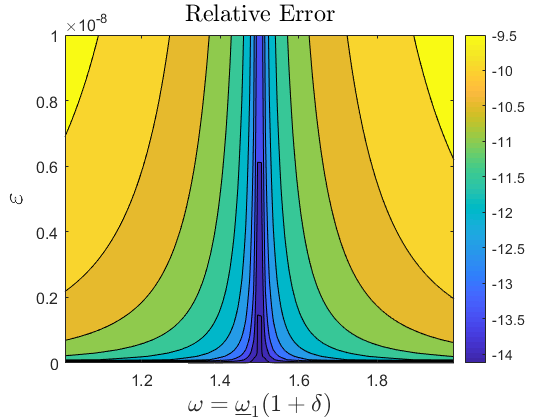
\includegraphics[width=7.6cm]{sections/5_method_of_maufactured_solutions/MMS_N_M_4_Upper_Field_Eps_1e-8.png} }}
%\includegraphics[width=0.5\textwidth]{conv_N}
\vspace{3mm}
\caption{Plot of relative error in the upper layer with fixed $N = M     = 4$
    and four choices of $\Eps = 10^{-2}, 10^{-4}, 10^{-6}, 10^{-8}$
    with Taylor summation.
    Physical parameters were $(5.27)$ and numerical
    discretization was $(5.28)$.}
\label{Fig:N}
\end{figure}
%
%\begin{figure}[hbt]
\vspace{-40mm}
\begin{figure}[H]
%\setcounter{figure}{14}
\centering
    \subfloat[\centering $N=M=4, \varepsilon=10^{-2}$ ]
    {{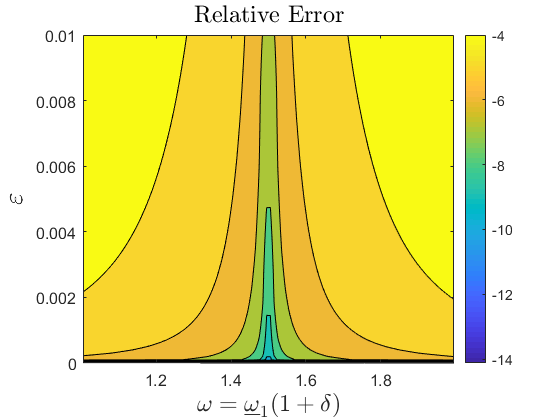
\includegraphics[width=7.6cm]{sections/5_method_of_maufactured_solutions/MMS_N_M_4_Upper_Field_Eps_1e-2.png} }}
    \subfloat[\centering $N=M=8, \varepsilon=10^{-4}$ ]
    {{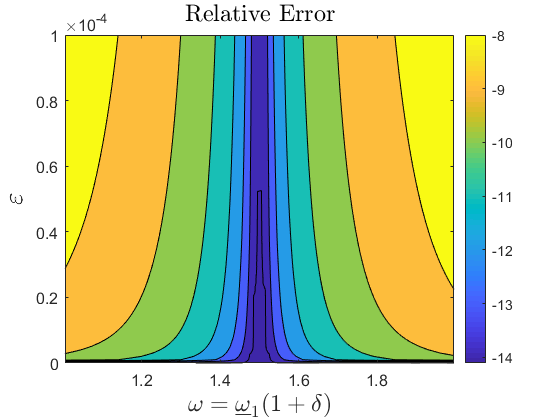
\includegraphics[width=7.6cm]{sections/5_method_of_maufactured_solutions/MMS_N_M_8_Upper_Field_Eps_1e-4.png} }}\\
    \subfloat[\centering $N=M=12, \varepsilon=10^{-6}$ ]
    {{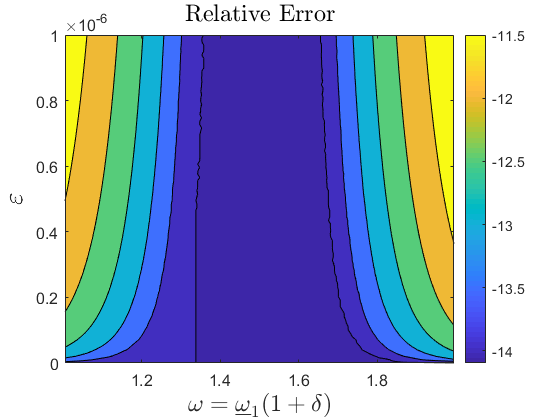
\includegraphics[width=7.6cm]{sections/5_method_of_maufactured_solutions/MMS_N_M_12_Upper_Field_Eps_1e-6.png} }}
    \subfloat[\centering $N=M=16, \varepsilon=10^{-8}$ ]
    {{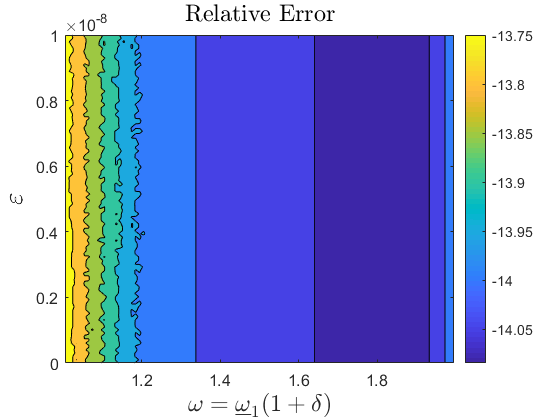
\includegraphics[width=7.6cm]{sections/5_method_of_maufactured_solutions/MMS_N_M_16_Upper_Field_Eps_1e-8.png} }}
%\includegraphics[width=0.5\textwidth]{conv_Eps}
\vspace{3mm}
\caption{Plot of relative error in the upper layer with four choices of $N = M = 4, 8, 12, 16$
    and four choices of $\Eps = 10^{-2}, 10^{-4}, 10^{-6}, 10^{-8}$
    with Taylor summation.
    Physical parameters were $(5.27)$ and numerical
    discretization was $(5.28)$.}
\label{Fig:Eps}
\end{figure}
\begin{flushleft}
\vspace{-20mm}
We then analyzed the lower lower--layer Dirichlet
data with the sinusoidal profile
\end{flushleft}
\be
\label{Eqn:Params:Geom:Lower}
g(x) = \Eps f(x) = \Eps \left( \frac{\sin(3 x)}{3} \right),
\ee
We used the following physical parameters
\be
d = 2 \pi,
\quad
\alpha = 0,
\quad
\epsilon^u = 1,
\quad
\epsilon^w = 1.1,
\quad
r = 8,
\quad
A_r = 4,
\quad
B_r = 5,
\label{Eqn:Params:Phys:Lower}
\ee
in TM polarization, and the numerical parameters
\be
\label{Eqn:Params:Num:Lower}
N_x = 32,
\quad
N_z = 32,
\quad
a = 1,
\quad
b = -1.
\ee
With these, we computed the relative error
\bes
\text{Error}_{\text{rel}} :=
  \frac{\SupNorm{\xi_r^{w,\text{exact}} - \xi_r^{w,\text{approx}}}}
  {\SupNorm{\xi_r^{w,\text{exact}}}}.
\ees
The results of our simulations are shown in 
Figures $15$ and $16$. More specifically,
Figure~$15$ displays both the rapid and stable decay of the 
relative error for fixed $N$ and $M$, and how this rate of decay
improves as $(\Eps,\delta)$ decrease. Figure~$16$ shows
both how the error shrinks as $(\Eps,\delta)$ become smaller, and that
this rate is enhanced as both $N$ and $M$ are increased.

\vspace{-13mm}
\begin{figure}[H]
\centering
    \subfloat[\centering $N=M=4, \varepsilon=10^{-2}$ ]
    {{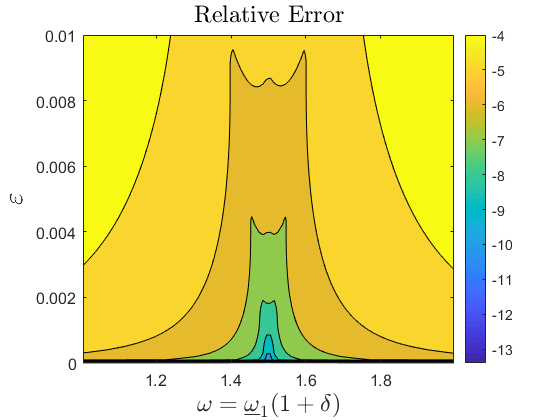
\includegraphics[width=7.6cm]{sections/5_method_of_maufactured_solutions/MMS_N_M_4_Lower_Field_Eps_1e-2.png} }}
    \subfloat[\centering $N=M=4, \varepsilon=10^{-4}$ ]
    {{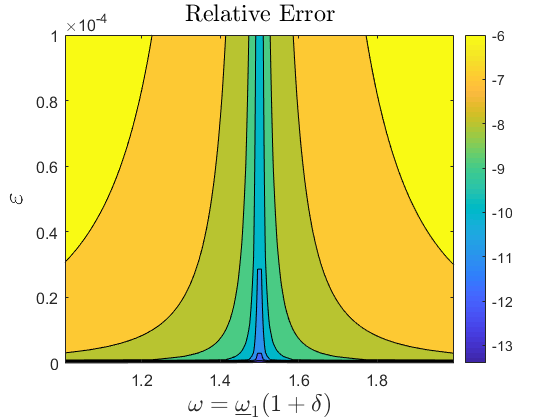
\includegraphics[width=7.6cm]{sections/5_method_of_maufactured_solutions/MMS_N_M_4_Lower_Field_Eps_1e-4.png} }}
    \\
    \subfloat[\centering $N=M=4, \varepsilon=10^{-6}$ ]
    {{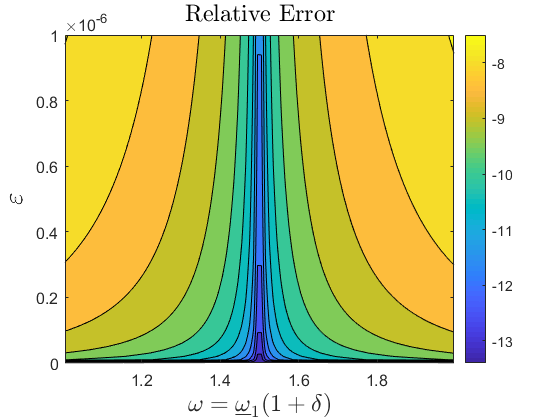
\includegraphics[width=7.6cm]{sections/5_method_of_maufactured_solutions/MMS_N_M_4_Lower_Field_Eps_1e-6.png} }}
    \subfloat[\centering $N=M=4, \varepsilon=10^{-8}$ ]
    {{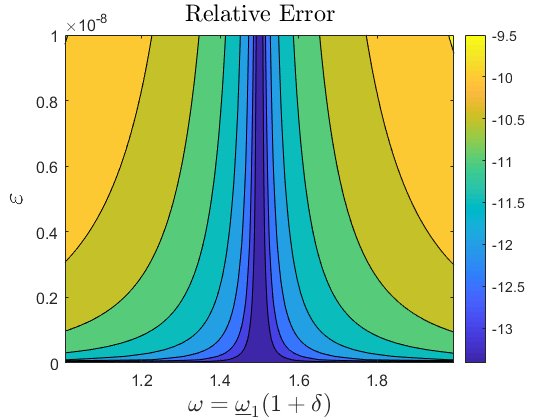
\includegraphics[width=7.6cm]{sections/5_method_of_maufactured_solutions/MMS_N_M_4_Lower_Field_Eps_1e-8.png} }}
%\includegraphics[width=0.5\textwidth]{conv_N}
\vspace{3mm}
\caption{Plot of relative error in the lower layer with fixed $N = M = 4$
    and four choices of $\Eps = 10^{-2}, 10^{-4}, 10^{-6}, 10^{-8}$
    with Taylor summation.
    Physical parameters were $(5.30)$ and numerical
    discretization was $(5.31)$.}
\label{Fig:N}
\end{figure}

%\vspace{-35mm}
%\begin{figure}[hbt]
\begin{figure}[H]
%\setcounter{figure}{16}
\centering
    \subfloat[\centering $N=M=4, \varepsilon=10^{-2}$ ]
    {{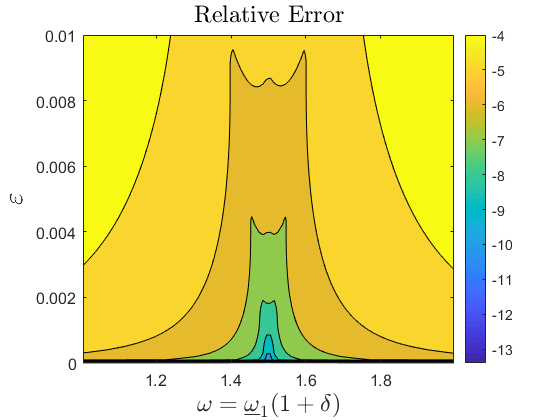
\includegraphics[width=7.6cm]{sections/5_method_of_maufactured_solutions/MMS_N_M_4_Lower_Field_Eps_1e-2.png} }}
    \subfloat[\centering $N=M=8, \varepsilon=10^{-4}$ ]
    {{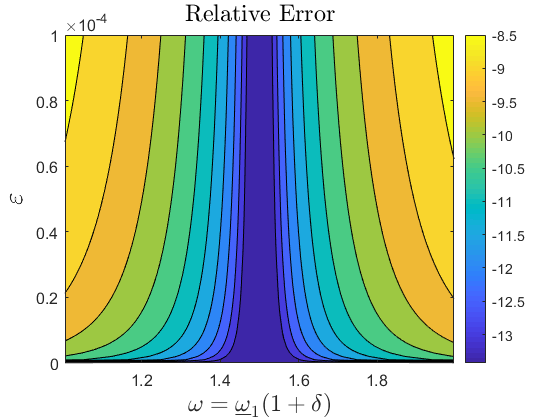
\includegraphics[width=7.6cm]{sections/5_method_of_maufactured_solutions/MMS_N_M_8_Lower_Field_Eps_1e-4.png} }}
    \\
    \subfloat[\centering $N=M=12, \varepsilon=10^{-6}$ ]
    {{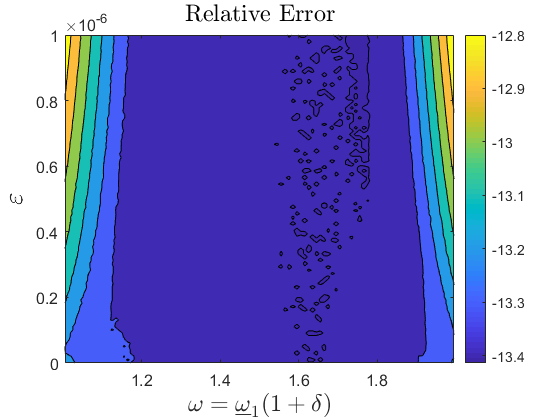
\includegraphics[width=7.6cm]{sections/5_method_of_maufactured_solutions/MMS_N_M_12_Lower_Field_Eps_1e-6.png} }}
    \subfloat[\centering $N=M=16, \varepsilon=10^{-8}$ ]
    {{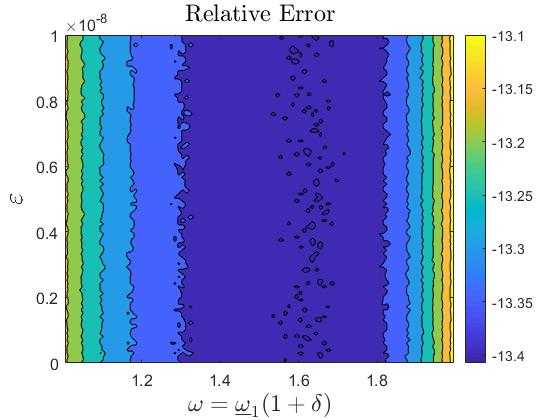
\includegraphics[width=7.6cm]{sections/5_method_of_maufactured_solutions/MMS_N_M_16_Lower_Field_Eps_1e-8.png} }}
%\includegraphics[width=0.5\textwidth]{conv_Eps}
\vspace{3mm}
\caption{Plot of relative error in the lower layer with four choices of $N = M = 4, 8, 12, 16$
    and four choices of $\Eps = 10^{-2}, 10^{-4}, 10^{-6}, 10^{-8}$
    with Taylor summation.
    Physical parameters were $(5.30)$ and numerical
    discretization was $(5.31)$.}
\label{Fig:Eps}
\end{figure}